%% Full length research paper template
%% Created by Simon Hengchen and Nilo Pedrazzini for the Journal of Open Humanities Data (https://openhumanitiesdata.metajnl.com)

\documentclass{article}
\usepackage{comment}
\usepackage[english]{babel}
\usepackage[utf8]{inputenc}
\usepackage{johd}

\title{Cloud Computing: A Revolutionizing Healthcare Management}

\author{Aditya Vikram Sharma,  Anchita Bose\\
        \small $^{*}$MSc Computer Science, St. Xavier's College(Autonomous), Kolkata \\\\
        \small \tt{adityavsharma1023@gmail.com,}
        \tt{anchitabose2002@gmail.com}
}

\date{} %leave blank

\begin{document}
\maketitle

\begin{abstract} 
\noindent Cloud computing is a fresh and rapidly expanding domain of progress within the healthcare industry. The combination of universally available, on-demand access to nearly limitless resources along with a pay-as-you-go approach enables novel methods of developing, delivering, and using services. Often used for computing in molecular medicine, genomics, and proteomics. Cloud computing has discovered fresh avenues in the storage, updating, and retrieval of electronic healthcare data originating from mobile and wearable healthcare sensors.
This paper presents an overview of the fundamental reasons and approaches for progressing towards a cloud-based e-healthcare system, along with potential challenges that might arise.
With technology improving every day, the traditional healthcare methodology is being replaced by smarter healthcare techniques.
At first, systems like the Healthcare Information System (HIS), and Electronic Health Records(EHR) were being used. However, these couldn't serve the purpose because of several issues like storage capacity, system integration, etc. To solve these issues, cloud computing came into action. Among the cloud services, SaaS is being widely used to cater to the readily changing needs of doctors and patients. 
\end{abstract}

\noindent\keywords{universally available; cloud computing;  molecular; sensors; e-healthcare; }\\

\begin{comment}
\noindent\authorroles{For determining author roles, please use following taxonomy: \url{https://credit.niso.org/}. Please list the roles for each author.} 
\end{comment}

\section{Introduction}

Healthcare is the provision of services by healthcare service providers to individuals or populations, to enhance, sustain, supervise, or recuperate health.
Globally, the ultimatum of healthcare is highly foreseeable, given its continuous projected growth in the future. This is attributed to factors like anticipated demographic changes within the aging population, the prevalence of lifestyle-related diseases, and increasing life expectancy.
Top-notch quality healthcare services include easy and quick accessibility along with affordability. It is the essential and appealing offer given by the healthcare sector in the current scenario.
Now this advancing development of the healthcare sector certainly gives rise to a huge quantity of patient data with a wide range of variety, and veracity and thus requires in turn a suitable infrastructure to maintain and enhance the high-quality reputation of a healthcare service provider. In general, this scenario presents two primary challenges for a healthcare system: increased complexity and a heightened demand for IT expertise.

Transitioning the healthcare sector to a cloud computing infrastructure to address this issue is unquestionably a promising solution. Cloud computing stands out among contemporary IT trends for its efficiency, business adaptability, and cost-saving potential. Consequently, this paper aims to present an overview of proposed healthcare architectures based on cloud solutions, along with the associated challenges in adopting this technology.

Embracing cloud technology offers the potential to realize two distinct objectives: the accessibility of e-health applications and medical data from any location and at any time, as well as the seamless integration of computing resources. These healthcare innovations have the capacity to facilitate a broad spectrum of applications and services, like mobile telemedicine, location-based medical services, patient monitoring, emergency response and management, ubiquitous access to healthcare information, and personalized monitoring. This holds significant advantages for both patients and medical professionals.

\subsection{Mobile Healthcare Systems And Cloud Computing}
Implementing health information management via mobile devices presents various hurdles. These include issues related to data storage and administration (such as physical storage limitations, availability, and maintenance), interoperability challenges arising from diverse resource availability, security, and privacy concerns (including permission controls and data anonymization), as well as the need for unified and widespread access.
Introducing the Cloud Computing concept in electronic healthcare systems acts as a one-shot solution to the above-mentioned problems since it provides the means to access shared resources and common infrastructure in a ubiquitous and pervasive fashion, providing on-demand services through the network to execute operations that align with evolving requirements in electronic healthcare applications.

\begin{figure}[H]
\centering
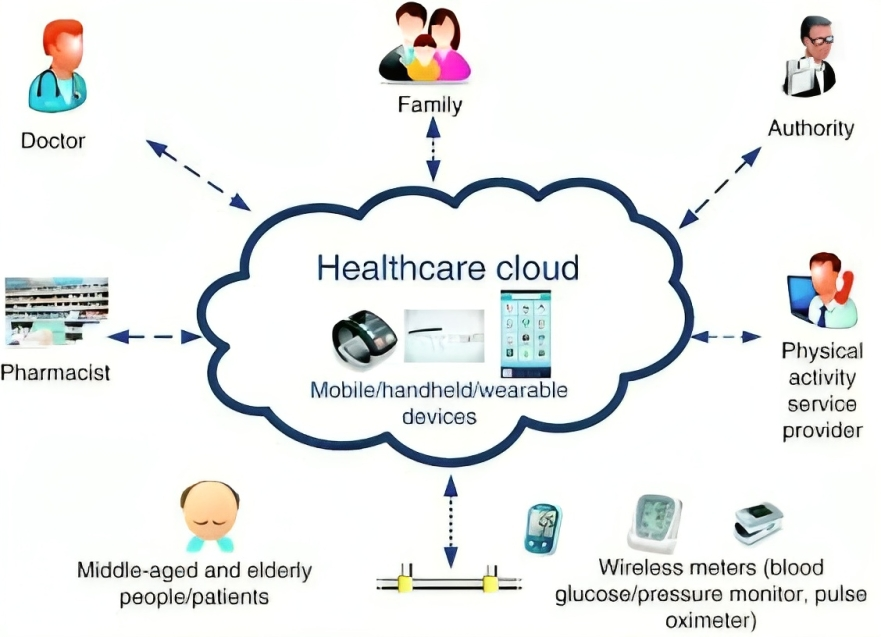
\includegraphics[width=0.5\textwidth]{images/mob.png}
\caption{\label{fig1}Mobile HealthCare Systems}
\end{figure}


\subsection{Implementing IoT and Cloud Computing towards Pervasive Healthcare} The adoption of the pervasive healthcare paradigm has heightened awareness about the independent living of elderly individuals and the necessity for continuous medical monitoring for chronic patients or individuals residing in remote, isolated areas.
 In this context, it is essential to ensure that advanced electronic healthcare services are accessible via a network at any time, from anywhere, and for anyone. 
On the contrary, a medical supportive environment involves the use of pervasive and omnipresent technologies to provide the mentioned services. Wireless technologies facilitate the real-time transmission of patient condition data to medical personnel.
There is a wide array of portable devices accessible that can ascertain specific medical conditions, such as pulse rate, breath alcohol level, blood pressure, and more, through contact with the user.

\section{Background Information}

Medicine is evolving into a progressively data-driven and cooperative field. The progress in OMICS disciplines, such as genomics and proteomics, generates substantial volumes of data that require processing and storage. Additionally, the secondary utilization of clinical data through text or data mining algorithms is leading to an escalating need for dynamic and scalable resources.
Frequently, these resources are employed temporarily, making it challenging to justify long-term infrastructure investments. As an alternative, flexible on-demand services are sought after. Cloud computing emerges as a viable solution to meet these requirements. Commercial providers such as Amazon and Microsoft pledge to provide access to hundreds of virtual machines almost instantly, and only for the duration they are genuinely required. The benefit of such offerings is that users are only charged for the specific configuration, size, and time they actually utilize(pay-per-use approach).

Consequently, the concept of "cloud computing" is defined by the National Institutes of Standards and Technology (NIST) as a framework that enables widespread, convenient, and immediate access to a shared, adaptable pool of computing resources. The key attributes of cloud computing, as outlined by Grance, encompass:

\begin{itemize}
    \item self-service provisioning
    \item extensive network accessibility
    \item resource consolidation with other users
    \item rapid scalability
    \item metered usage tracking.
\end{itemize}

Cloud computing offers benefits in terms of dynamic resource allocation, such as computing power and storage capacity, as well as the ability to access resources from anywhere at any time. Additionally, it provides high levels of flexibility and scalability. These advantages have driven the growing adoption of cloud computing in various business sectors. Notably, in recent years, this concept has also made its way into the healthcare domain.

Upon examining the extensive body of recent literature focused on cloud solutions in healthcare, it becomes evident that a significant portion of these reports predominantly discusses the use of cloud computing technologies as a substitute for grid computing in the OMICS field. Conversely, other domains of application, such as health information systems, health information exchange, or image processing and management, appear to receive comparatively less attention.

\section{Current Healthcare System's Issues} Healthcare systems primarily include services for both individual patients and the general public, as well as educational and research endeavors. IT solutions have greatly benefited healthcare by reducing human errors, enabling agile access and processing of extensive patient data, and conserving paper and storage space. The rapid advancements in smart electronic devices have further enhanced the dynamic nature of healthcare delivery.
Nonetheless, present-day electronic healthcare systems continue to grapple with challenges related to cost, connectivity, client support, and disaster recovery. The introduction of flexible IT infrastructure and ongoing advancements in smart electronic devices have raised concerns regarding their compatibility with existing healthcare systems.
For instance, data generated by implantable biomedical devices for home healthcare monitoring needs to be stored in the healthcare organization's database, allowing healthcare professionals to promptly and accurately assess patients' conditions at home. However, current technologies like distributed and grid computing fall short of addressing the dynamic, scalable, and cost-effective requirements of both existing and emerging healthcare applications.
Efficiently managing and maintaining these extensive datasets is critical to these organizations' success, as their IT hardware and software require regular maintenance, monitoring, and skilled personnel for upgrades. Furthermore, healthcare organizations' on-premises data is susceptible to both environmental and human threats.

\medskip

\section{Brief Overview of Cloud Computing}
A typical definition of cloud computing describes it as a paradigm that allows universal and convenient access to a shared pool of adaptable computing resources, including storage, applications, networks, servers, and services. Furthermore, cloud computing operates with minimal management effort or interaction with service providers, boasting its distinct set of standards and practices.

The five crucial aspects of cloud computing are:
\paragraph{On-demand Self-Service:} A consumer or client in the realm of cloud computing can independently access computing resources, such as server time and network storage, as needed without the need for direct human interaction with the service provider.

\paragraph{Broad network access:} The capabilities of this technology are accessible via the network and can be accessed through standard mechanisms supported by various client platforms, including both lightweight and robust clients, such as mobile devices and workstations.

\paragraph{Resource pooling:}  Providers cater to a multitude of consumers, and computing resources are consolidated using a multi-tenant model, allowing for the dynamic allocation and reallocation of various physical and virtual resources in response to consumer needs. This occurs without the need for direct control or awareness of the exact location of the allocated resources, except at a higher level of abstraction.

\paragraph{Rapid elasticity:}  Cloud Computing also possesses the capability to flexibly allocate and release resources, expanding or contracting in response to demand, sometimes even automatically. The ability to provision resources limitlessly and for the appropriate duration is a significant and critical concern for consumers, in particular.

\paragraph{Measured service:} Cloud computing systems autonomously manage and enhance resource allocation by measuring capacity at a certain level of abstraction to accommodate a range of services. Typically, this is achieved through a pay-as-you-go model. Both providers and consumers can oversee, regulate, and report resource usage, thereby creating a mutually transparent environment for both parties.

\begin{figure}[H]
\centering
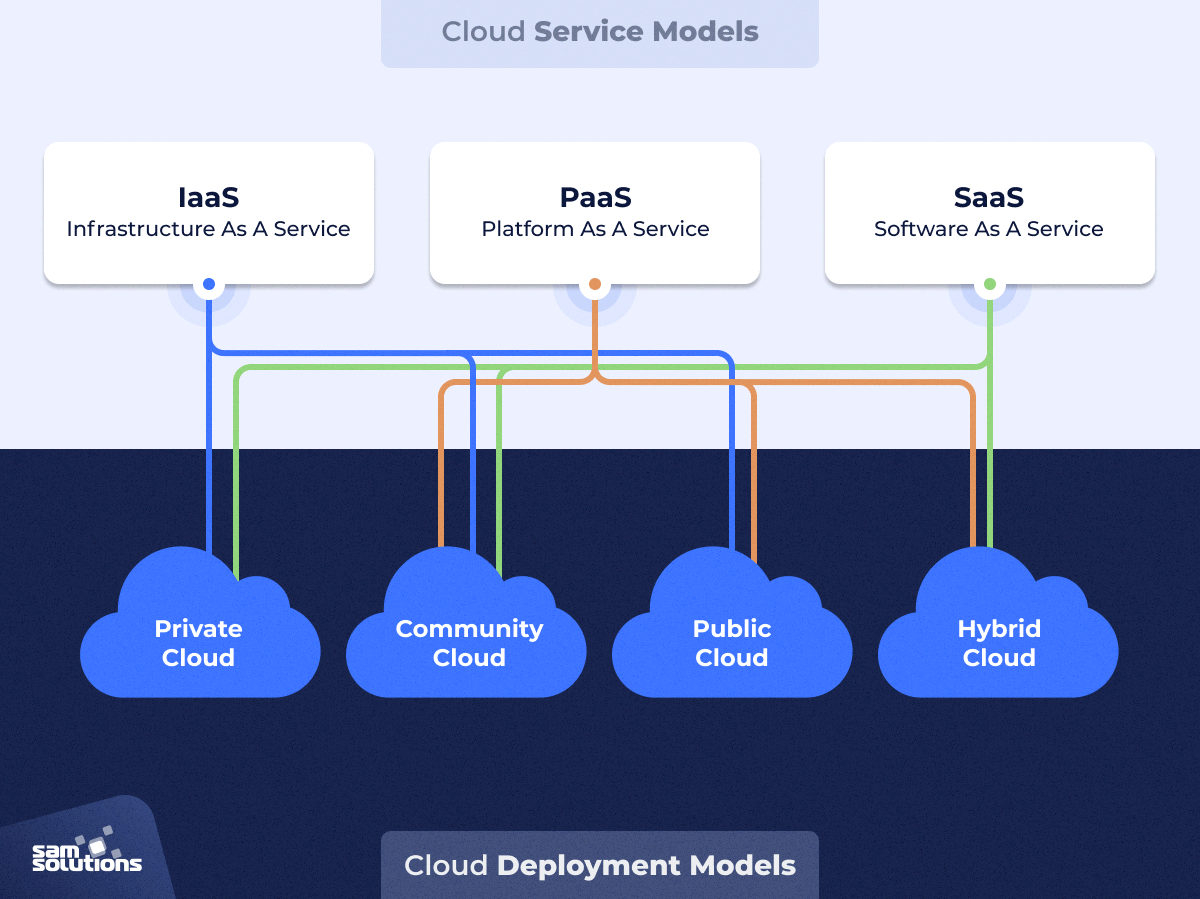
\includegraphics[width=0.5\textwidth]{images/csm.png}
\caption{\label{fig2}Cloud Service Models}
\end{figure}


\subsection{Service Models}
The relationship between operating costs and flexibility is closely tied to the service models. These factors exhibit an inverse correlation, where Software as a Service (SaaS) has the lowest operating costs, followed by Platform as a Service (PaaS), and Infrastructure as a Service (IaaS). This results in greater flexibility in IaaS, followed by PaaS and SaaS.

\paragraph{Software as a Service (SaaS):} The service offered to the client involves utilizing applications developed by the host, which are readily accessible on a cloud infrastructure. Infrastructure components such as networks, servers, storage, operating systems, and even the functionalities of individual applications are typically not under the direct management of the consumer or client, except for specific application configuration settings, which may be adjusted by a limited set of users.

\paragraph{Platform as a Service (PaaS):} The consumer has the ability to deploy applications onto the cloud infrastructure, whether these applications are created by the consumer themselves or obtained from external sources. These applications are developed using programming languages, libraries, services, and tools provided by the service provider. However, the consumer does not oversee or direct the underlying cloud infrastructure, which includes components like the network, servers, operating systems, and storage. Instead, they maintain control over the deployed applications and may have the option to configure settings within the application hosting environment.

\paragraph{Infrastructure as a Service (IaaS):} This service facilitates the configuration of processing, networking, and storage resources to ensure computing capabilities in an environment where end users are distributed, enabling the installation of various software, including operating systems and applications. Unlike the other two services, the consumer does not have direct control over the cloud infrastructure. Instead, they manage frameworks, storage, and application setups, with limited control over certain networking components like host firewalls.

\subsection{Deployment Models}
Four types of models deployed under cloud computing: 

\paragraph{1. Public Cloud:} This form of cloud infrastructure is made available for public use, typically managed and operated by corporate, academic, or government organizations, or a combination of these entities who own it. Users pay based on their usage, allowing them to scale resources up or down according to the service level agreement, to accommodate varying demands, whether they increase or decrease.

\paragraph{2. Private Cloud:}
A private cloud's infrastructure is dedicated solely to the use of a single organization with multiple consumers. This infrastructure can be owned, managed, and operated by the organization itself, a third party, or a combination of both, and it may be located either on or off the organization's premises. Because it serves only one organization, there is greater flexibility in enforcing compliance requirements related to data ownership and privacy.

\paragraph{3. Community Cloud:} This model is specifically crafted to cater to a community of consumers who share common interests, such as mission and policies within their organizations. The ownership, management, and operation of this cloud can be entrusted to a third party, one or more organizations from the same community, or a combination of these entities. This cloud type can be located either on or off-premises. The concept of sharing within this model often means that organizations within the community tend to have similar security, privacy, performance, and compliance requirements. However, it also serves as a boundary, preventing participation from organizations outside of the same industry or with differing desires.

\paragraph{4. Hybrid Cloud:} The hybrid cloud infrastructure is formed by integrating two or more separate cloud infrastructures mentioned earlier into a single cohesive entity. These clouds are interconnected using standardized or proprietary technology, enabling the seamless transfer of data and applications between them.

\section{The Rise of Cloud in Healthcare} Cloud technology not only enhances healthcare practices but also fosters innovation, enabling smart healthcare to reach patients in both rural and urban areas, including those facing challenging circumstances.
Transitioning to smart healthcare necessitates the creation of personalized management strategies that empower patients to take control of their advanced health information, fostering collaborative care through creative technology utilization. Many previous studies reported the potential benefits of cloud computing.
Among these approaches, Rolim et al introduced a cloud-based system for automating the collection of patients' vital data through a network of sensors linked to traditional medical devices. This data is then sent to a medical center's cloud for storage, processing, and distribution. The system offers continuous, real-time data collection throughout the week, reducing the need for manual data collection and minimizing the risk of typing errors, simplifying deployment. Numerous articles and resources also reported the successful application of cloud computing in bioinformatics research. Harvard Medical School's Center for Biomedical Informatics Laboratory for Personalized Medicine harnessed cloud computing advantages to create genetic testing models that efficiently processed vast data volumes in record time.

The American Occupational Network is enhancing patient care by digitizing health records and modernizing clinical procedures with cloud-based software from IBM Business Partners, and MedTrak Systems. This has enabled them to accelerate and improve billing for both individuals and insurance companies, reducing the time to generate a bill from 7 days to under 24 hours and cutting medical transcription expenses by 80\%.


\section{Related Work}
Now that we have a basic understanding of cloud deployment and service models let us talk about the application of mobile devices for pervasive healthcare information management.
 We recognize the advantages of employing virtual health records to support the mobile healthcare of senior citizens. The primary objective is to establish a smooth and uninterrupted flow of communication between home healthcare services and primary care providers, facilitated by devices such as PDAs and Tablet PCs. Electronic storage of patient records has been implemented through the utilization of smart cards and web interfaces.

The MADIP system represents a decentralized information platform designed for extensive health data sharing through mobile agents. In this context, we introduce a mobile platform designed to facilitate the exchange of medical images and patient records across wireless networks, employing advanced compression techniques. Most of the previous initiatives mentioned are built upon exclusive architectures and communication methods, necessitating the installation of specialized software components.
Moreover, the studies predominantly emphasize the delivery of data to healthcare applications, neglecting to tackle the challenges associated with data management and interoperability arising from the diverse data sources present in contemporary healthcare systems. The adoption of Cloud Computing offers solutions for data management and access, effectively addressing the aforementioned challenges, as outlined in earlier sections. While the integration of Cloud Computing in healthcare information management is a relatively recent concept, it is widely regarded as having significant potential.

Now let us talk about some cloud-based services designed specifically for the storage of sensor-derived data. Numerous research studies focus on pervasive healthcare sensors. Many of these studies concentrate on managing data within the devices, such as through storage solutions like SD cards, or they make use of intermediary nodes like mobile phones or directly store the data on computer nodes. However, there are only a limited number of works that specifically tackle the challenge of data storage and management in the Cloud. The platform introduced in this context is proprietary, and the initial evaluation results are derived from simulated sensors rather than real devices.
Conversely, there is currently a range of cloud-based services designed specifically for the storage of sensor-derived data. Some notable examples include Nimbits, iDigi, ThingSpeak, and Pachube.

\paragraph{Pachube} in particular, stands out as one of the pioneering online database service providers that enable developers to link sensor data to the internet. This platform functions as a real-time cloud-based infrastructure, offering support for the Internet of Things (IoT) concept.
To provide a more detailed description, it can be characterized as a scalable framework that empowers individuals to create IoT products and services. Additionally, it facilitates the storage, sharing, and exploration of real-time data related to sensors, the environment, and energy from objects, buildings, and devices worldwide. The primary functionalities of this platform encompass the management of real-time sensor and environmental data, as well as the capabilities for monitoring, graphing, and remotely controlling environments.
Furthermore, there exists a wide array of interfaces accessible for the development of sensor or mobile-driven applications tailored for data management on the Cloud infrastructure. An essential factor contributing to Pachube's widespread adoption as an IoT cloud service is its complimentary basic usage, reliance on an open and readily accessible API, and the presence of an exceptionally interactive website for overseeing sensor data.

\paragraph{Nimbits} is a cloud-based service designed to capture and distribute sensor data. It serves as a social, open-source platform tailored for the Internet of Things (IoT). In Nimbits, sensor data is saved as data points, which can utilize textual, JSON, or XML values. These data points can be customized to execute computations, trigger notifications, share data on social networks, and integrate with SVG process control diagrams, spreadsheets, and websites. Nimbits also incorporate features like data compression, alert management, and the ability to perform data calculations using straightforward mathematical formulas on the incoming sensor data.

\paragraph{ThingSpeak} is also an open-source application tailored for the "Internet of Things" (IoT), offering developers access to APIs for the storage and retrieval of data from sensors and devices via HTTP on the Internet. Users can develop a variety of applications for logging sensor data, tracking locations, and establishing a social network of interconnected devices with status updates. Beyond just storing and retrieving numeric and alphanumeric data, the ThingSpeak API also enables numeric data manipulation, including tasks like time scaling, averaging, finding the median, summing, and rounding. Each ThingSpeak Channel accommodates entries for up to 8 data fields, along with latitude, longitude, elevation, and status information. These channel feeds support various formats, including JSON, XML, and CSV, for seamless integration into applications.

\paragraph{The iDigi system} serves as a platform-as-a-service designed for machine-to-machine (M2M) communication. This platform aims to simplify the process of creating secure, scalable, and cost-efficient solutions that effectively link enterprise applications with device assets. iDigi handles the communication between enterprise software and remote device assets, regardless of their location or the network they are connected to. It streamlines the task of connecting remote assets by providing a comprehensive set of tools for establishing, overseeing, storing, and transmitting data across different parts of the enterprise. Additionally, iDigi facilitates the management of products, including ZigBee nodes, through tasks such as configuration, upgrades, monitoring, analysis, and alarming.

\begin{figure}[H]
\centering
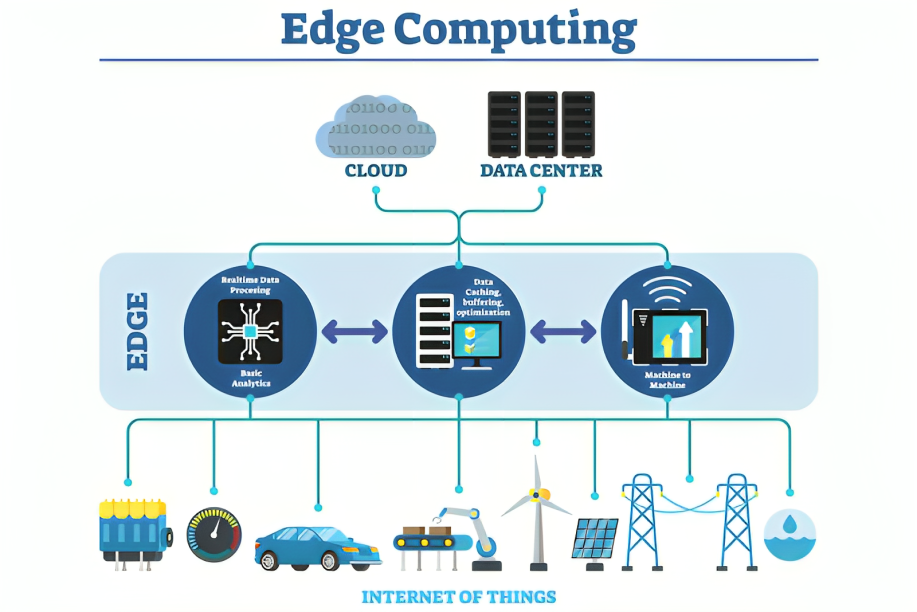
\includegraphics[width=0.6\textwidth]{images/edge.png}
\caption{\label{fig3}Edge Computing}
\end{figure}

\section{Integrating Cloud Technology In Healthcare}
Numerous research projects have explored the use of cloud computing as an IT solution to enhance healthcare services. For instance, in the work of C. Rolim et al, they introduced a cloud-based system designed to automate the collection of patients' vital data through a network of sensors linked to electronic medical devices. This system aims to transmit the data to cloud storage for real-time processing and distribution. However, the paper did not provide further information about the mechanisms ensuring trust and privacy protection.

DACAR (Data Capture and Auto Identification Reference project): 
The goal of this project make it highly secure in the cloud computing infrastructure for healthcare data and also storage. To ensure data privacy, DACAR employs a private cloud for data storage and utilizes a hybrid cloud for hosting its services. 
DACAR comprises five steps:
\begin{itemize}
    \item[1.] Patients initiate the process by entering their username and password.
    \item[2.] These credentials are then forwarded to a Single Point of Contact (SPOC) for verification to determine whether the patient is authorized to request the service.

    \item[3.] If the user is granted permission, the SPOC generates a Service Ticket. However, if access is denied, the system sends an error message along with the reason for the denial.

    \item[4.] In the final step, authorized users are free to utilize the service.
\end{itemize}

\bigskip
\bigskip
\bigskip

As the demand for digitization in healthcare continues to surge, leading competitors in this space include:
\begin{itemize}
    \item[1.] Practo (enables doctor-patient connectivity, digital record-keeping, billing, and reminders).
    \item[2.] DocSuggest (helps users find suitable doctors and schedule appointments via website or phone calls).
    \item[3.] Mocdoc (provides appointment booking, SMS reminders, follow-up calls, and digital record-keeping).
    \item[4.] SmartRx (offers appointment booking, access to patient records, and alerts for diagnostics and consultations).
\end{itemize}

\section{Cloud Service} 
Cloud computing has led to enhanced collaboration among doctors, patients, and hospitals. Smart healthcare systems possess predictive capabilities and can make decisions while interacting with their surroundings. Additionally, they have the potential to operate autonomously in terms of energy and are interconnected. The pressing requirement for widespread and constant real-time access to patient data from any location and using any digital device is crucial for accurate diagnosis and treatment procedures, ultimately resulting in the delivery of high-quality medical services. The cloud services provided by organizations come with both advantages, disadvantages, and associated challenges, as outlined below:
\subsection{Benefits} Introducing cloud technology in businesses not only reduces the need for server management staff but also lowers the requirement for servers, resulting in reduced power consumption.
\paragraph{Enhanced Performance:} The health cloud offers the potential for improved patient care by facilitating the seamless sharing of unified patient records with other medical specialists when necessary. These digital records are accessible anytime, anywhere, providing a comprehensive view of the patient's medical history.

\paragraph{Reduced Maintenance:} Cloud services alleviate the need for hardware and software maintenance in enterprises. Organizations no longer handle or manage the software, allowing them to concentrate on essential tasks without incurring extra IT staffing and training expenses.

\paragraph{Projection:} The health cloud can aid strategic decision-makers in planning and budgeting for healthcare services. Its integrated approach can assist in forecasting future healthcare requirements.

\subsection{Challenges} 
\paragraph{Sufficient Bandwidth:} To upload and download data from the cloud, it's crucial to have the appropriate bandwidth. Given the large size of medical data, sufficient bandwidth is essential for seamless data access.
\paragraph{Cultural Resistance:} Commonly, there is cultural resistance, when it comes to sharing data and transitioning from traditional work methods, which poses a management challenge in adopting cloud computing.
\paragraph{Data lock-in:} It presents a significant challenge as well. There are situations where cloud users may need to transfer data or services either to a different provider or back to an in-house IT setup due to the cessation of business or service operations by the current provider.


\section{Mobile Application Overview} In this section, we will discuss the main features of the HealthCloud application along with its implementation details. The primary purpose of the application is to offer medical professionals and patients a mobile user interface for handling healthcare information. This encompasses tasks such as storing, searching for, and retrieving medical images, patient health records, and medical data related to patients (such as biosignals). This data may be located in a distributed Cloud Storage facility, initially uploaded and stored by medical staff through a Hospital Information System (HIS).
To ensure compatibility with various Cloud Computing infrastructures, it's essential to engage in communication and data exchange using communication standards that are not proprietary and are open and interoperable. HealthCloud, which utilizes Web Services connectivity and the Android OS, facilitates the following capabilities: \\

\textbf{It enables a smooth connection to Cloud Computing storage:} The primary application empowers users to access, edit, and upload medical content like medical images, patient health records, and biosignals by leveraging Web Services and the REST API.
The content is stored in distributed storage components at a remote location, but the user experiences it as if the resources were available locally on their device. \\

\textbf{Patient Health Record Management:} The application's interface allows for the display and management of information related to patient health records, including the patient's status, associated biosignals, and image content. \\

\textbf{Image viewing support:} The application provides support for the DICOM medical image protocol and incorporates the JPEG2000 standard to enable both lossy and lossless compression. This implementation covers advanced coding techniques, including progressive coding and Region of Interest (ROI) coding. Progressive coding allows users to decode large image files at various resolution levels, optimizing the use of network resources. This means that even in scenarios with limited network availability, image acquisition remains possible. Additionally, modifications have been made to the code for wavelet decoding on mobile devices to ensure compatibility with the JPEG2000 standard on the Android platform. The application also offers image annotation functionality, making use of the multi-touch features of the Android OS.\\

\textbf{Proper user authentication and data encryption:}  Authentication of the user on the Cloud Computing Service involves SHA1 hashing for message authentication and SSL for securing data communication through encryption.

\begin{figure}[H]
\centering
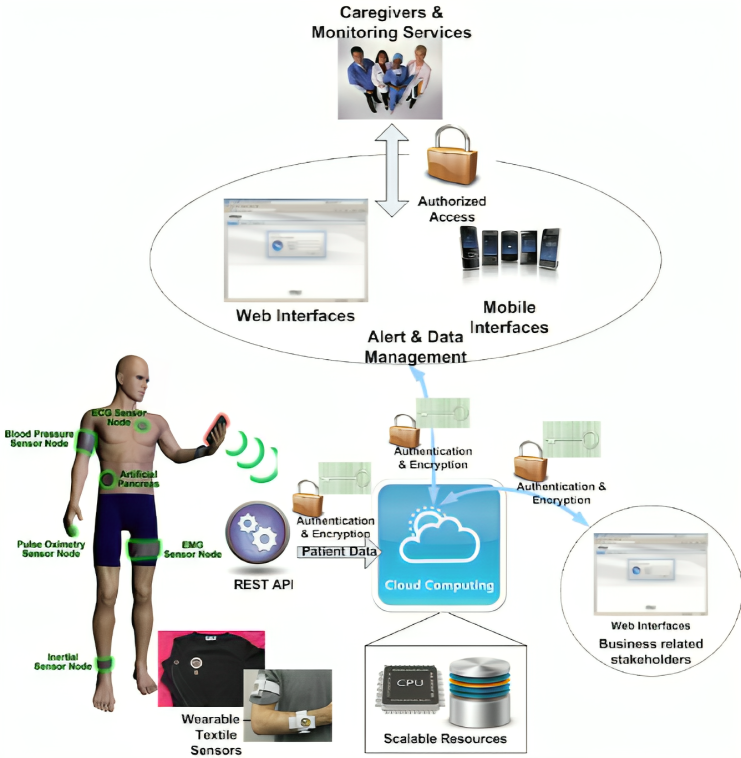
\includegraphics[width=0.6\textwidth]{images/arc.png}
\caption{\label{fig4}Proposed Application Architecture}
\end{figure}

\section{Proposed System Architecture And 
Implementation Details
} The healthcare industry stands apart from other sectors, with its distinctive characteristics falling into three main categories. Firstly, it is subject to extensive regulation and legal oversight, primarily aimed at ensuring patient safety. Secondly, the potential cost of errors and risks in healthcare is significantly higher compared to other industries. Lastly, this sector comprises a multitude of units, including hospital administrative staff, laboratories, and patients. Taking these points into account we proceed with the system architecture.
Cloud computing not only decreases the expenses associated with these systems in terms of ownership and IT upkeep but also provides the benefits of facilitating the sharing, integration, and management, making the tracking of patients and diseases more efficient and effective.
\subsection{
System architecture for mobile healthcare applications}
In this subsection, we talk about the system architecture for developing mobile healthcare applications that utilize cloud computing. Typically, a Cloud Computing Service consists of two primary elements. Firstly, there's the frontend interface, which directly interacts with users and enables them to manage the content stored in the cloud. This interface can take the form of a web client or a standalone application. Secondly, there are the Cloud Storage Facilities, which oversee the physical infrastructure, including storage components, and carry out essential maintenance tasks such as data backup. The Cloud Platform interface is linked to the Cloud Service module, which takes care of managing and queuing user requests. Additionally, the Cloud Infrastructure module is responsible for handling user accounts, accessibility, and billing matters. Prior research has shown that mobile devices can effectively retrieve medical image data from remote repositories wirelessly by using suitable content encoding techniques, such as wavelet compression with region of interest support. This research has now been expanded to encompass the ability to communicate with Cloud Computing platforms and facilitate communication through Web Services.

In this context, HealthCloud was created using Google's Android mobile Operating System (OS) with a suitable software development kit (SDK). Android is a mobile OS built on the Linux kernel and is already supported by numerous mobile device manufacturers. This platform is versatile, accommodating both larger and standard smartphone designs, and it offers compatibility with various connectivity technologies like CDMA,  UMTS, EV-DO, WiFi, and Bluetooth. HealthCloud is compatible with a wide range of audio, video, and still image formats, making it well-suited for the presentation of medical content. Additionally, it harnesses native multi-touch technology, enhancing the manipulation of medical images and overall improving the application's user-friendliness.
The Cloud Service client operating on the Android OS comprises multiple modules. 
\begin{itemize}
    \item \textbf{The Patient Health Record application} is responsible for retrieving and presenting patient records stored in the cloud
    \item \textbf{The Medical Imaging module} is tasked with displaying medical images on the device.
\end{itemize}

It deciphers images stored in DICOM format, presenting both the image itself and the associated textual data. When JPEG2000 compression is applied, a dedicated sub-module takes care of decoding the image. Interaction with the Cloud is carried out through the implementation of a Web Services REST API, which is natively supported by Android. The built-in interoperability, thanks to the use of XML technologies that are independent of vendors, platforms, and programming languages, along with the widespread use of HTTP as a transport method, means that any application can communicate seamlessly with another using Web services. Data stored in the Cloud is seamlessly accessible to the user, giving the impression that it exists locally. This setup presents the Cloud repository as a virtual folder rather than a conventional database system. To offer the user data querying capabilities, medical records and associated data such as images and biosignals are stored within a SQLite file.

Android supports the use of SQLite as its database platform. The file is stored in a designated location in the cloud and is retrieved whenever the user needs to access data. Queries are performed locally and applications are given access to the data without revealing its exact location in the cloud. Any modifications made by the user are updated in the database file and uploaded to the cloud.

\begin{table}[H]
\centering % Label your table accordingly

\caption{\label{tab1}Transmission Time of Medical Images Amazon S3 Cloud}
\begin{tabular}{cccc}
\hline\hline
\textbf{Image Type (encoding)}  & \textbf{File Size(MB)} & \multicolumn{2}{c}{\textbf{Time (Secs)}}  \\
\textbf{} & \textbf{} & \textbf{3G network} & \textbf{Wifi Network}\\\hline
OT (24-bit JPEG2000\\ 
Lossless Color) & 6.8 & 42.532 & 7.894\\\\
CT(Uncompressed) & 0.528 & 4.023 & 2.382\\\\
CT(JPEG2000) & 0.102 & 1.223 & 0.892\\\\
MR(JPEG Lossless) & 0.721 & 9.738 & 3.894\\\\
Ultrasound(seq of\\10 imgs, JPEG2000) & 0.487 & 3.892 & 3.251\\
\hline\hline
\end{tabular}
\end{table}

\hfill
\subsection{IoT-based System Architecture for managing Sensor Data} This sub-section discusses the proposed IoT-based architecture for acquiring and managing sensor data on the Cloud.
The fundamental elements within the suggested architecture encompass:
\begin{itemize}
    \item The wearable and mobile sensors responsible for collecting patient biosignals, motion data, and contextual information.
    \item The sensor gateway aggregates signals from the sensors and transmits them to the Internet. This gateway can be a mobile phone or a microcontroller platform equipped with internet communication capabilities. Additionally, it relays information concerning the sensors' status, such as their operational condition and power source levels.
    \item The Cloud platform offers communication APIs, which are streamlined interfaces, such as REST Web Services. These interfaces are accessible to the sensor gateways for transmitting sensor data and retrieving information. Additionally, external applications can utilize these APIs for tasks like data processing, billing, alert management, and more.
    \item The management application comprises a web-based platform that operates in real-time and offers visual representations of sensor data, such as graphs, along with critical details regarding the patient's context, such as their location and activity status.
    \item The Cloud infrastructure serves as the hosting environment for the interfaces and the management application. Within this infrastructure, it supplies the necessary resources such as CPU, storage, and application servers. These resources are utilized for deploying the web application and the interfaces, which facilitate communication with the sensors and various external systems.
\end{itemize}

\section{Conclusion}
The utilization of e-Health Cloud technology offers an efficient solution for numerous healthcare providers grappling with concerns like rising healthcare delivery costs, limited healthcare professionals, and the need for improved information sharing. Cloud computing enables healthcare organizations to shift their focus towards enhancing the quality of healthcare services, rather than managing their own IT infrastructure. It also streamlines information sharing among various healthcare institutions involved in the treatment process, a critical aspect of healthcare delivery.
When a healthcare organization contemplates transitioning its services to the cloud, it must engage in strategic planning. This planning involves assessing various environmental factors such as staffing, budget, technologies, organizational culture, and government regulations that could impact the transition. Organizations also need to evaluate their capabilities in achieving this goal and devise strategies to move forward effectively. By implementing best practices in the design, deployment, and utilization of cloud technology, there is hope for the widespread adoption of cloud-based systems in the future, despite the challenges that may arise.

The advent of cloud computing platforms has shifted the traditional PC-centric environment towards a culture centered around documents. The healthcare sector faces immense challenges in providing high-quality services to patients and healthcare professionals worldwide. Information technology (IT) emerges as a solution to address the demanding and fast-paced healthcare requirements. A health cloud is conceived as a network of numerous computers and servers specifically tailored to fulfill the healthcare industry's demands. It has brought about significant changes in the storage and accessibility of information.

\begin{comment}
\subsection{In-text citations}
This journal uses a style based on the APA system (see \href{https://openhumanitiesdata.metajnl.com/about/submissions/#References}{here}). \\
The following are some basic citation commands in \LaTeX: \\

\noindent
\verb|\citet| $\rightarrow$ \citet{jenset&mcgil}\\
\verb|\citet| $\rightarrow$ \citet{australiashealth}\\
\verb|\citet| $\rightarrow$ \citet{shree-a}\\
\verb|\citep| $\rightarrow$ \citep{fabricius-hansen2012b}\\
\verb|\citealp| $\rightarrow$ (\citealp{eckhoff2018a})\\
\verb|\citealp| $\rightarrow$ (\citealp{eckhoff2018a}; \citealp{fabricius-hansen2012b}; \citealp{shree-a})\\

\subsubsection{Other simple functions}
To add bullet points:

\begin{itemize}
    \item Some point
    \item Another point
\end{itemize}

\noindent Or numbered points:

\begin{itemize}
    \item[1.] Some numbered point
    \item[2.] Another numbered point
\end{itemize}

\noindent This is an example of footnote\footnote{This is a footnote}. \\

\noindent This is a simple table:


\noindent Please refer to your table using: Table \ref{tab1}.\\

\noindent To add a figure, upload the figure into the \texttt{images} folder, and then embed it:

\begin{figure}[H]
\centering
\includegraphics{images/image.jpeg}
\caption{\label{fig1}JOHD's logo.}
\end{figure}

\noindent To resize the figure:

\begin{figure}[H]
\centering
\includegraphics[width=0.2\textwidth]{images/image.jpeg}
\caption{\label{fig2}JOHD's logo.}
\end{figure}

\begin{figure}[H]
\centering
\includegraphics[width=0.8\textwidth]{images/image.jpeg}
\caption{\label{fig3}JOHD's logo.}
\end{figure}

\noindent Please refer to your figures as: Figure \ref{fig1}, Figure \ref{fig2}, etc.


\section{Dataset description}
Here you can provide, if applicable, information about the dataset(s) whose creation, collection, management, access, processing, or analysis have been discussed in this paper, following this schema:
\paragraph{Object name} Typically the name of the file or file set in the repository.
\paragraph{Format names and versions} E.g., ASCII, CSV, Autocad, EPS, JPEG, Excel, SQL, etc.
\paragraph{Creation dates} The start and end dates of when the data was created (YYYY-MM-DD).
\paragraph{Dataset creators} Please list anyone who helped to create the dataset (who may or may not be an author of the data paper), including their roles (using and affiliations).
\paragraph{Language} Languages used in the dataset (i.e., for variable names etc.).
\paragraph{License} The open license under which the data has been deposited (e.g., CC0). 
\paragraph{Repository name} The name of the repository to which the data is uploaded. E.g., Figshare, Dataverse, etc. 
\paragraph{Publication date} If already known, the date in which the dataset was published in the repository (YYYY-MM-DD).

\section{Method}
Describe the methods used in the study.

\section{Results and discussion}
Describe and discuss the results of the study.

\section{Implications/Applications}
Provide information about the implications of this research and/or how it can be applied.
\end{comment}

\bibliographystyle{johd}
\bibliography{ref}
\cite{pdf1}
\cite{pdf2}
\cite{pdf3}
\cite{pdf4}
\cite{pdf5}
\cite{pdf6}
\cite{pdf7}
\cite{pdf8}
\cite{pdf9}
\cite{pdf10}
\end{document}